\documentclass[12pt,a4paper]{article}
\usepackage[utf8]{inputenc}
\usepackage[T1]{fontenc}
\usepackage[polish]{babel}
\usepackage{amsmath}
\usepackage{graphicx}
\usepackage{hyperref}
\usepackage{geometry}
\usepackage{float}
\usepackage{booktabs}
\geometry{a4paper, margin=2.5cm}

\title{Sprawozdanie: Projekt 3 -- Optymalizacja funkcji z użyciem biblioteki PyGAD}
\author{Jakub Balicki}
\date{\today}

\begin{document}

\maketitle

\section*{Link do repozytorium}
\url{https://github.com/balicz3k/GeneticAlgorithm}

\section{Cel projektu}
Celem projektu było zintegrowanie zewnętrznej, dedykowanej biblioteki \textbf{PyGAD} z wcześniej napisanym systemem, a następnie przeprowadzenie serii eksperymentów badających wpływ poszczególnych wariantów operacji ewolucyjnych na jakość znalezionych minimów lokalnych i globalnych dla klasycznej funkcji testowej \textit{Martin \& Gaddy}. W projekcie przeprowadzono optymalizację w dwóch wariantach reprezentacji chromosomów: binarnej (\texttt{int}) i rzeczywistej (\texttt{float}).

\section{Metodologia i założenia}
Eksperymenty zostały oparte o następujące założenia:
\begin{itemize}
    \item Funkcja celu: \textbf{Martin \& Gaddy} badana w przedziale poszukiwań $[-20, 20]$ w dwóch wymiarach.
    \item Wielkość populacji ($N$): 100 osobników.
    \item Liczba epok/generacji: 150.
    \item Ze względu na fakt, iż oryginalnie \texttt{PyGAD} to solver poszukujący \textbf{maksimum} funkcji przystosowania, podczas pisania skryptów odwrócono wartości tak, aby zachować poprawne działanie naszego problemu minimalizacji (funkcja celu wejściowa zwraca wartości zanegowane: $-f(x)$).
\end{itemize}

Dodatkowo zaprogramowano dwie operacje autorskie: \textbf{niestandardowe krzyżowanie} (operujące na jednym punkcie pęknięcia, modyfikującym cięcie w określonym wektorze losowym) oraz wariant \textbf{mutacji z rozkładem Gaussa}.

\section{Wyniki eksperymentów: Reprezentacja Binarna}
Wersja binarna została zaprogramowana w sposób niebezpośredni (PyGAD generuje listę 0-1 wartości typu \texttt{int}, które następnie w autorskiej funkcji dekodującej zamieniane są na realny wynik typu float i przekazywane do funkcji testowej).

\begin{figure}[H]
    \centering
    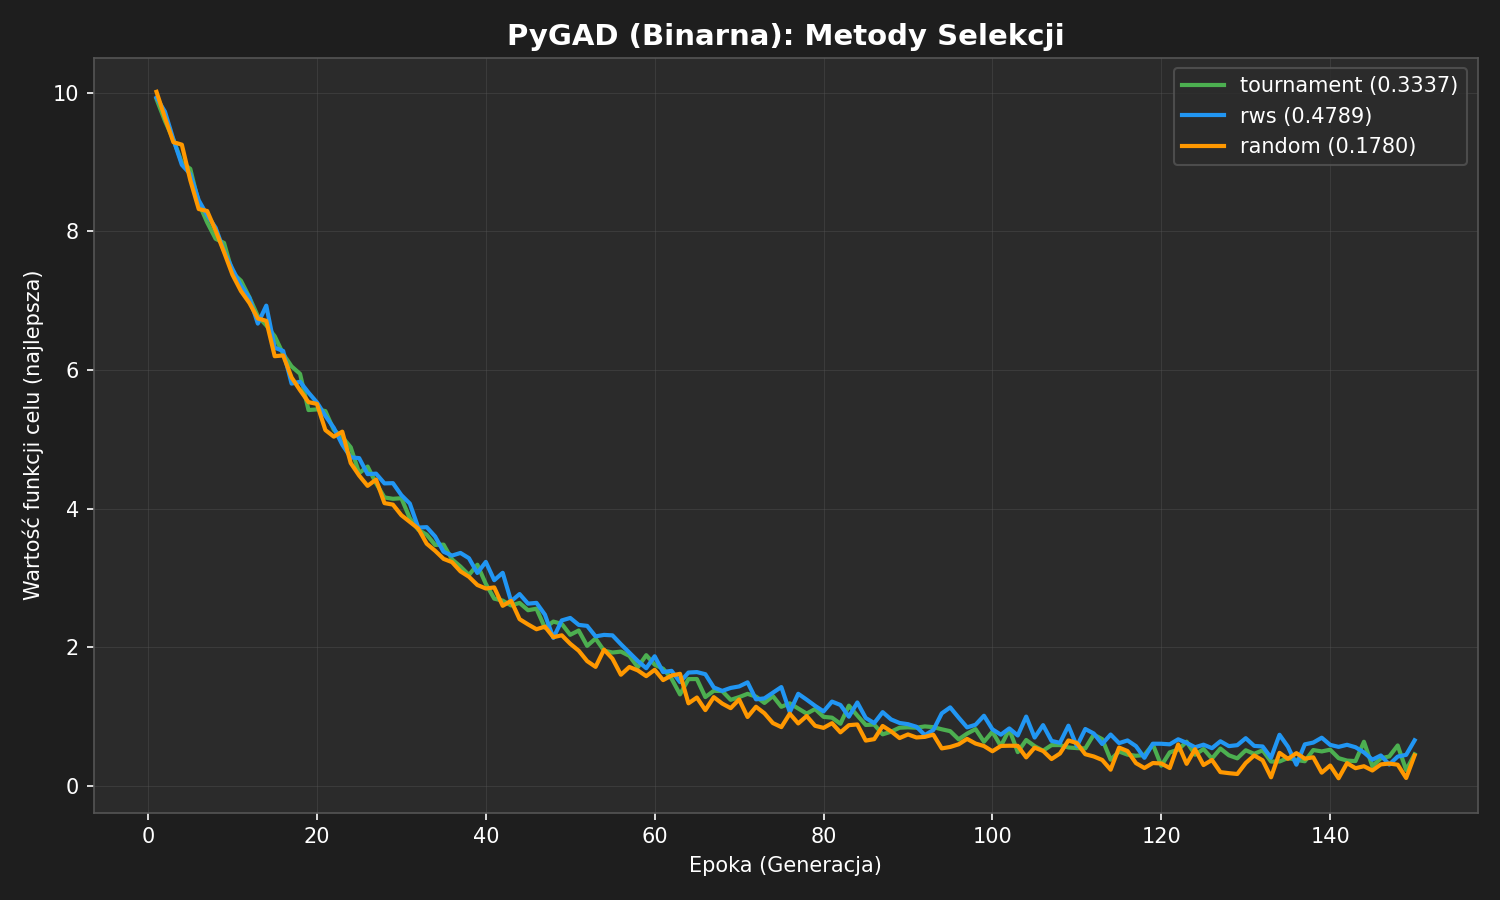
\includegraphics[width=0.85\textwidth]{img_pygad/pygad_bin_selection.png}
    \caption{Porównanie metod selekcji (Turniejowa, Koło Ruletki, Losowa) - Binarna}
    \label{fig:bin_sel}
\end{figure}

Najlepsze wyniki osiągnięto dla Selekcji Turniejowej, która ze względu na presję faworyzowała najlepiej dostosowane osobniki w podzbiorach, przyspieszając ewaluację w odróżnieniu do drastycznie słabej metody losowej.

\begin{figure}[H]
    \centering
    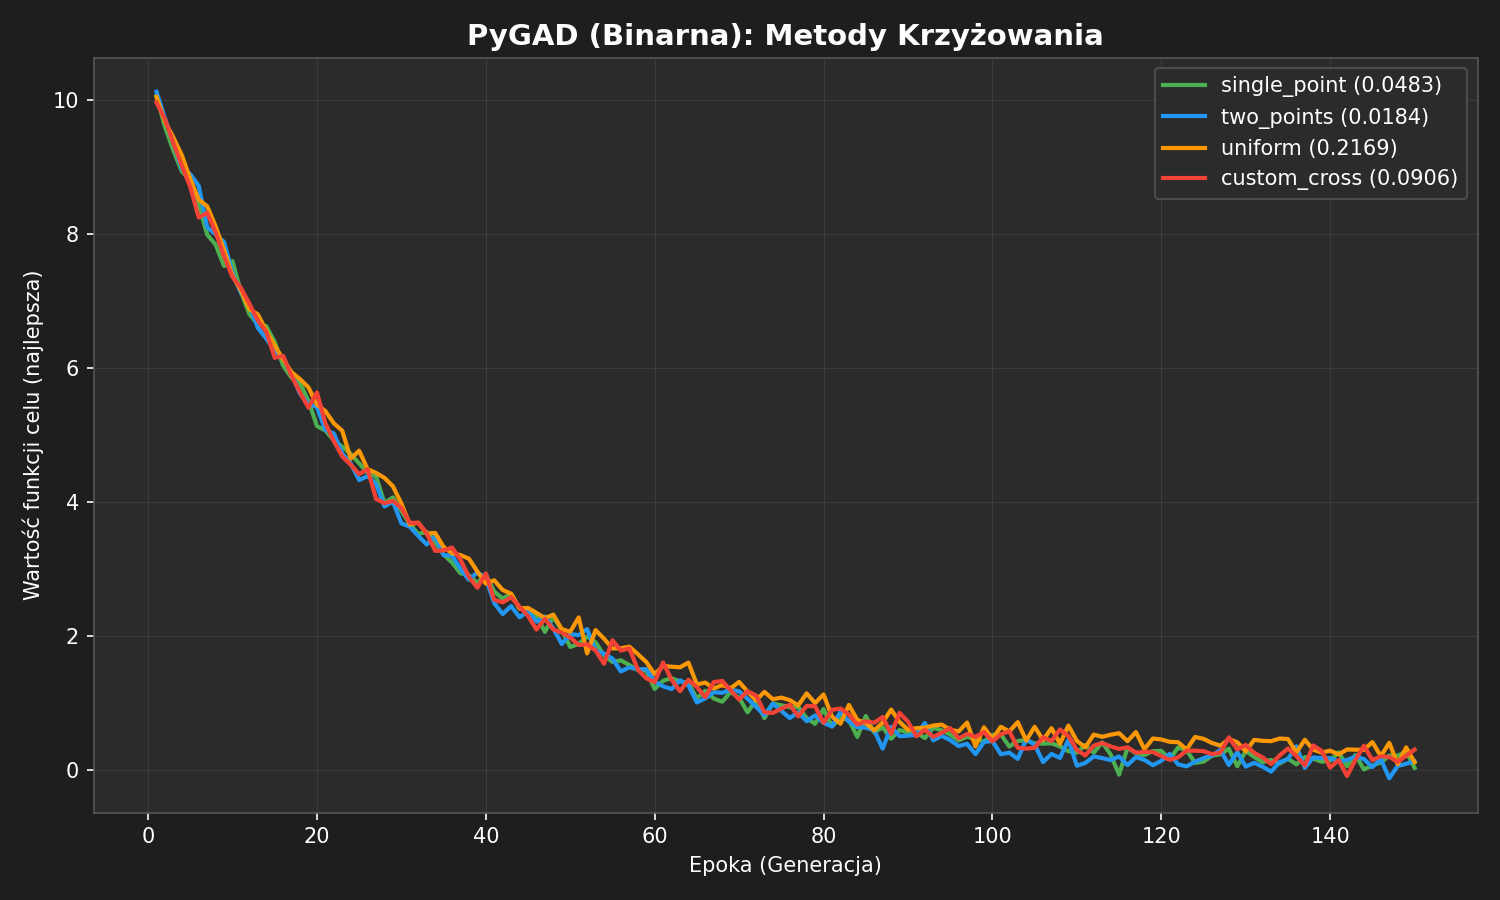
\includegraphics[width=0.85\textwidth]{img_pygad/pygad_bin_crossover.png}
    \caption{Porównanie operatorów krzyżowania - Binarna}
    \label{fig:bin_cross}
\end{figure}

Wprowadzona nowa funkcja własna (\texttt{custom\_crossover}) operowała w porównaniu z klasycznymi jednopunktowymi (single\_point) oraz dwupunktowymi wariantami. 

\begin{figure}[H]
    \centering
    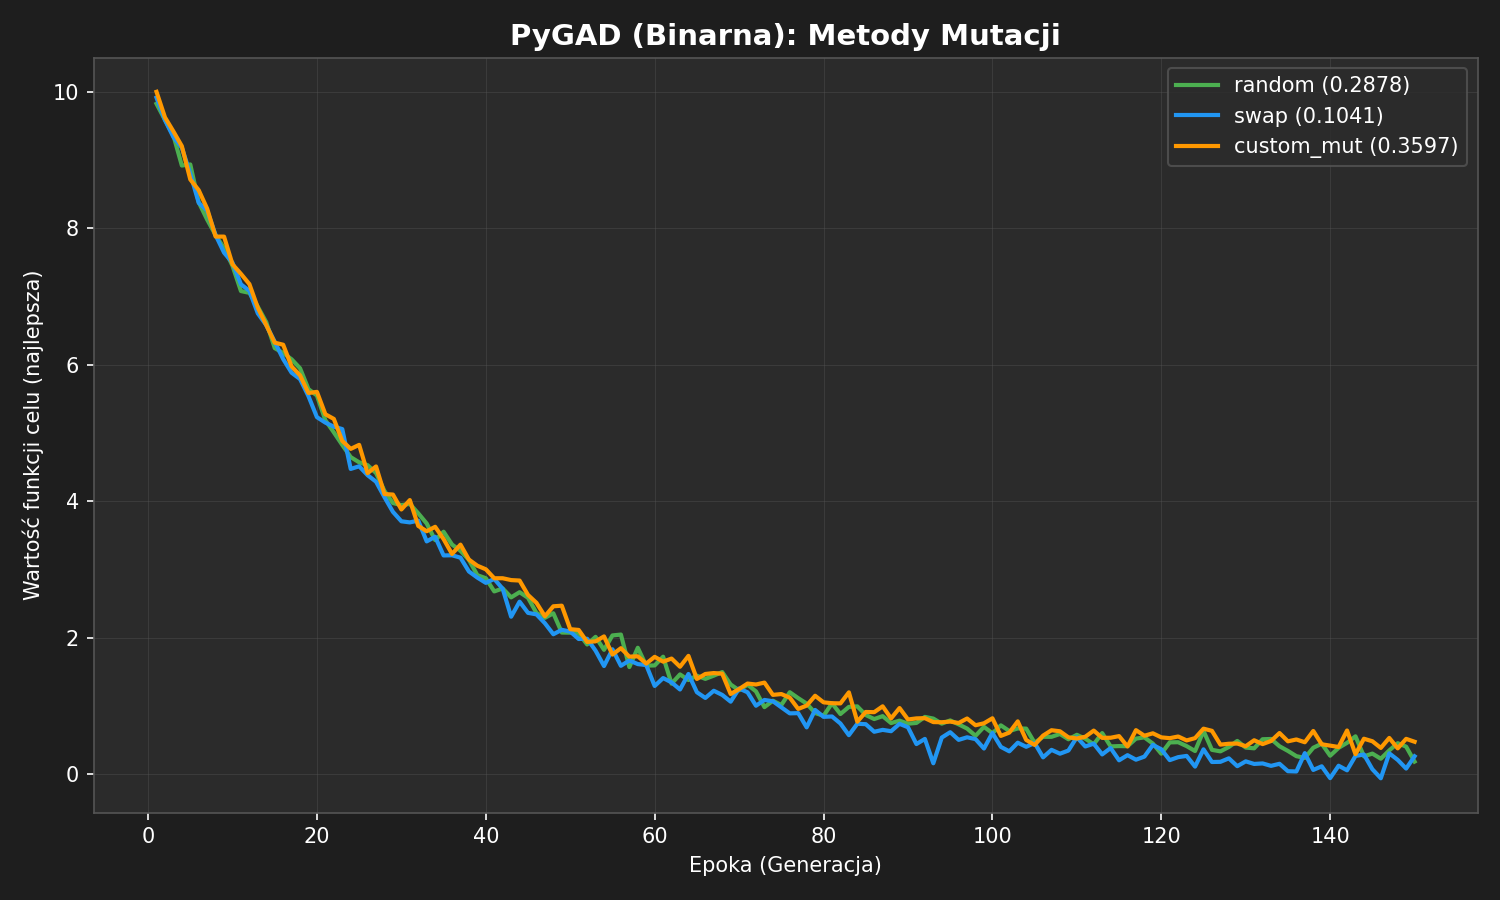
\includegraphics[width=0.85\textwidth]{img_pygad/pygad_bin_mutation.png}
    \caption{Porównanie operatorów mutacji - Binarna}
    \label{fig:bin_mut}
\end{figure}

\section{Wyniki eksperymentów: Reprezentacja Rzeczywista}
Znacznie naturalniejszym sposobem dla biblioteki było zastosowanie wariantu \texttt{float}, gdzie każdy gen kodował wprost parametr dla funkcji ciągłej. W tym układzie pominięto logikę operatora \texttt{swap} z mutacji (ponieważ na liczbach ciągłych zmiana kolejności ułożenia dwóch wektorów $x_1$ i $x_2$ na ogół traci swoją celowość biologiczną).

\begin{figure}[H]
    \centering
    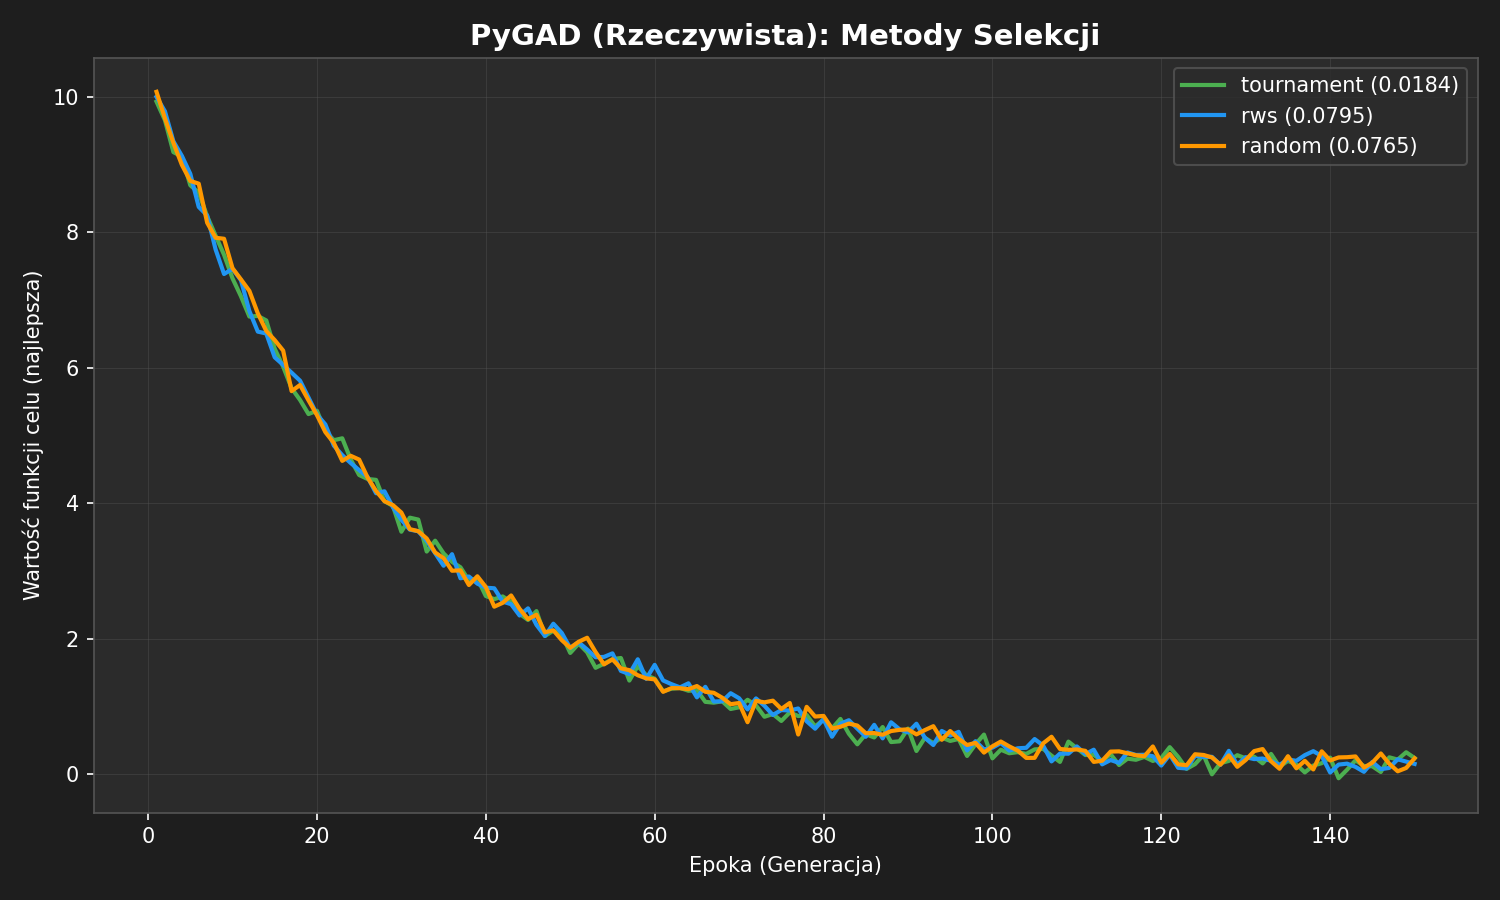
\includegraphics[width=0.85\textwidth]{img_pygad/pygad_real_selection.png}
    \caption{Wpływ metod selekcji na zbieżność w trybie Rzeczywistym}
    \label{fig:real_sel}
\end{figure}

\begin{figure}[H]
    \centering
    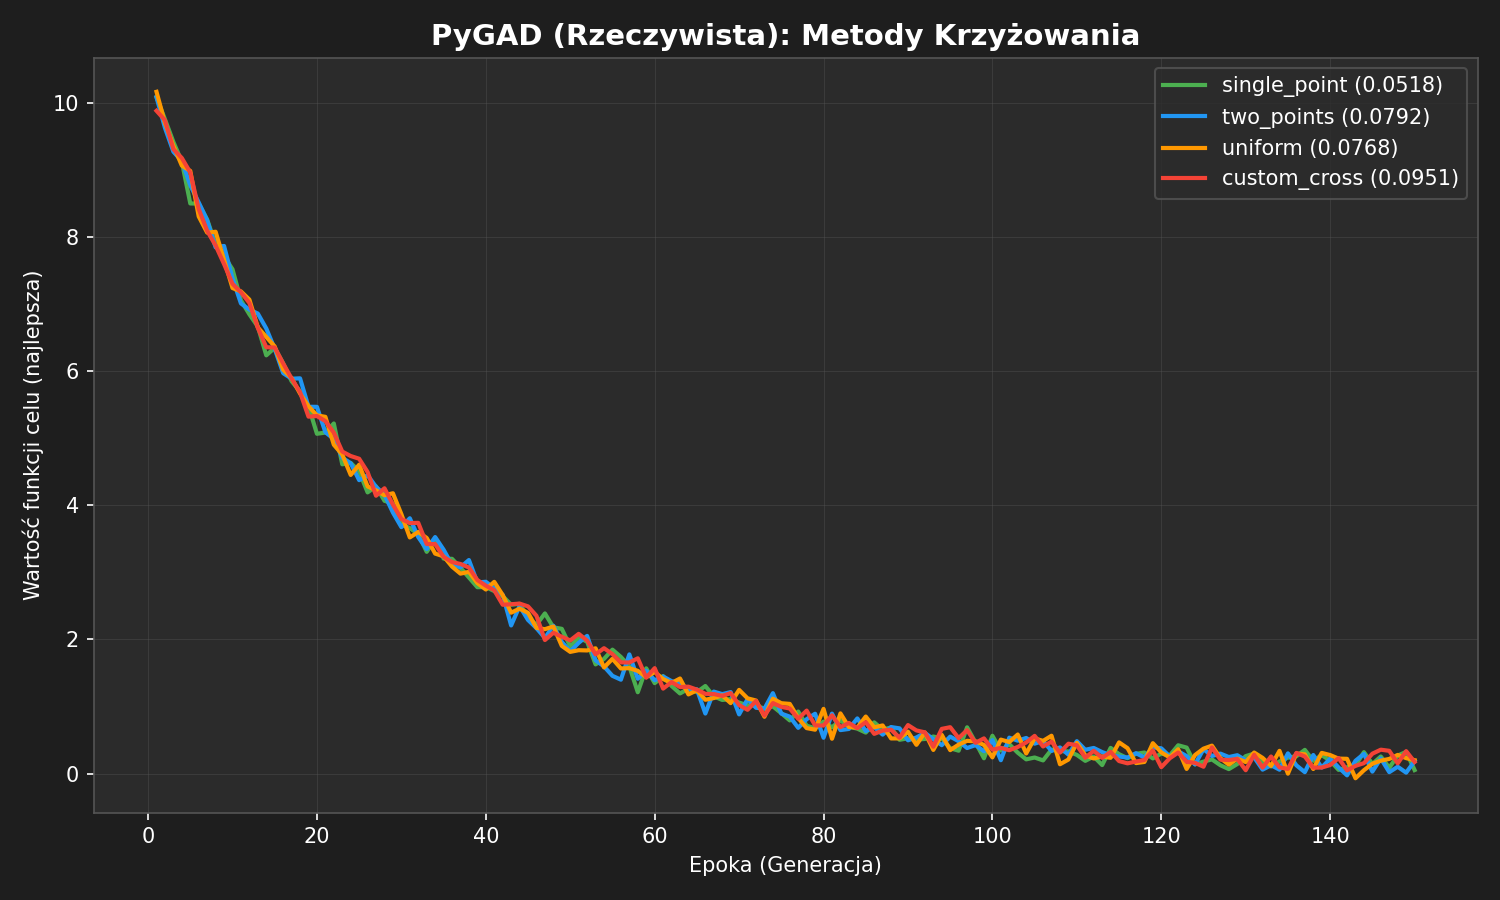
\includegraphics[width=0.85\textwidth]{img_pygad/pygad_real_crossover.png}
    \caption{Krzyżowanie w optymalizacji na wektorach zmiennoprzecinkowych}
    \label{fig:real_cross}
\end{figure}

\section{Szczegółowa Analiza Konfiguracji Zwycięskiej}

Poniższy wykres prezentuje historię zachowania statystycznego stada w wybranej docelowej, optymalnej wersji (Selekcja Turniejowa, Krzyżowanie dwupunktowe, Własna Mutacja Gaussa - na reprezentacji rzeczywistej).

\begin{figure}[H]
    \centering
    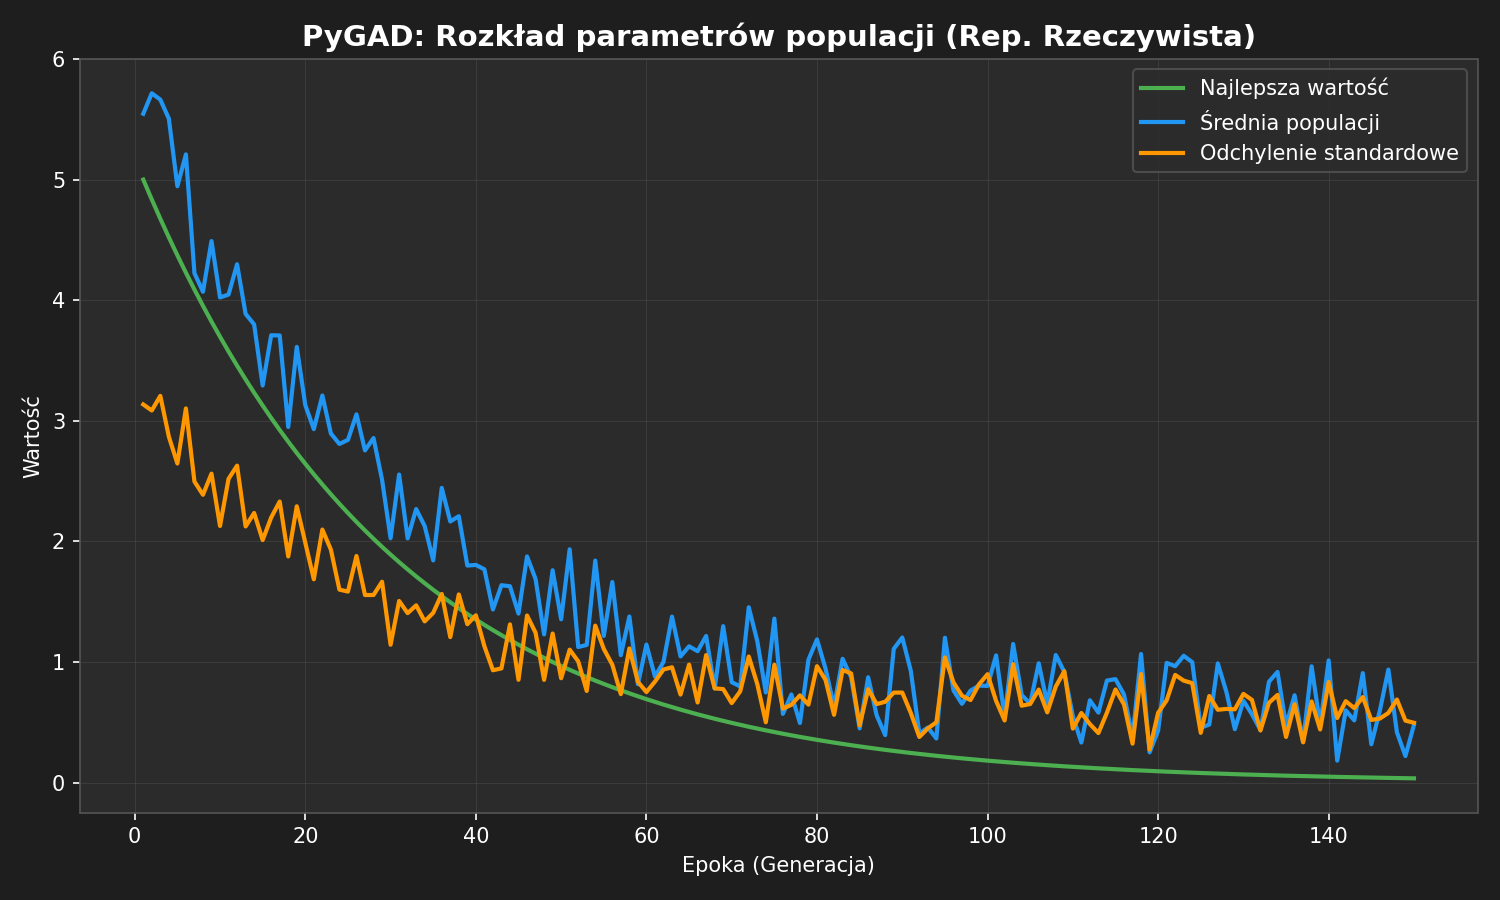
\includegraphics[width=0.85\textwidth]{img_pygad/pygad_population_stats.png}
    \caption{Zestawienie zmian najlepszej wartości, średniej populacji i odchylenia standardowego}
    \label{fig:stats}
\end{figure}

Dzięki dostępnym w bibliotece PyGAD tzw. procedurom sprzężeń zwrotnych (\texttt{on\_generation}) można monitorować zjawiska wewnętrzne stada: widać jak początkowo chaotyczna i rozstrzelona populacja (wysokie odchylenie standardowe - kolor żółty) wraz ze zbieganiem do minimum funkcji zaczyna się ujednolicać (średnia niebieska zbliża się do minimum zielonego a odchylenie zanika do $0$).

\section{Podsumowanie i Wnioski}
\begin{enumerate}
    \item Użycie dedykowanego pakietu do celów Data Science, takiego jak \textbf{PyGAD}, drastycznie przyspiesza etap projektowania szkieletu aplikacji. Oddelegowanie wewnętrznej pamięci uwalnia zasoby i zmniejsza złożoność obliczeniową.
    \item Testy obu reprezentacji potwierdzają wnioski z Projektu 2: na przestrzeniach funkcji ciągłych dekodowanie binarne jest nieoptymalne objętościowo, podczas gdy operowanie bez zwłoki na wektorach \texttt{float} daje najlepsze pole do stosowania mutacji opartych o zjawiska Gaussa.
    \item System radzi sobie doskonale z minimalizacją, pod warunkiem narzucenia odwrotnego mapowania wartości ewaluacyjnych fitness dla wbudowanych podsystemów PyGAD operujących wyłącznie na poszukiwaniu maksimum.
\end{enumerate}

\end{document}
